\section{Stochastic Fast}
\label{sec:1STF}

Stochastic Fast - wskaźnik stochastyczny szybki, zaproponowany w latach 50-tych przez George C. Lane. Sposób wyliczenia wartości wskaźnika uwzględniając wartości O,H,C,L, polega na wyliczeniu dwóch linii. \ref{wzor_1} oraz \ref{wzor_2}.
\begin{equation}
ValK=100*[ \frac{C-Min(L;n)}{max(H;n - min(L;n)}]
\label{wzor_1}
\end{equation}
\begin{equation}
ValD=EMA(ValK;3)
\label{wzor_2}
\end{equation}
gdzie:
\begin{itemize}
\item ValD - jest wygładzoną linią ValK
\item n - ilość dni
\item EMA - Wykładnicza średnia krocząca(Exponential Moving Average)
\end{itemize}

\noindent Do podstawowych własności wskaźnika należą:
\begin{itemize}
\item opokazuje poziom dzisiejszego zamknięcia w stosunku do najniższego oraz najwyższego punktu w badanym okresie
\item porusza się w przedziale od 0-100
\item obliczamy 2 linie oscylatora ValK i ValD (Value K i Value D) uwzględniając, że ValK jest główną linią oscylatora natomiast ValD jest wygładzoną postacią ValK
\end{itemize}
Najważniejszą własnością opisywanego wskaźnika, stosowaną przy implementacjach strategii, jest fakt wskazywania momentów w których powinny zostać zawarte transakcje. 
\begin{itemize}
\item sygnałem kupna jest przecięcie linii ValK ponad ValD
\item sygnałem sprzedaży jest przecięcie linii ValK poniżej ValD.

\end{itemize}
\noindent Poniższy listing przedstawia zaimplementowaną strategię w środowisku MATLAB.
\begin{scriptsize}
\begin{lstlisting}
[a b]=size(C);
roz=(60*a)/100;
roz=round(roz);
paramSectionLearn = C(1:roz,:);

[m,n]=size(paramSectionLearn);

O=paramSectionLearn(:,1);
L=paramSectionLearn(:,3);
H=paramSectionLearn(:,2);
C=paramSectionLearn(:,4);

%Parametry 
spread=0.00016;
bestReturn = -100;
bestMa = 0;
%Część ucząca

countCandleLearn=m;
lastCandleLearn=0;
krok=1;
%Część valid

paramALengthT=0;
countCandleTest=m1;
lastCandleTest=0;
tmp=countCandleLearn-1;
ValK=zeros(1, countCandleLearn);
paramZakrespocz=0;
chwi=1;
for paramALengthL=40 %liczba świec wstecz ( do max)
        chwi=chwi;
        chwi
    paramZakrespocz(chwi)=paramALengthL;
   for i=2:tmp
       max3=max(H(max(i-paramALengthL, 1):i));
       min3=min(L(max(i-paramALengthL, 1):i));
      ValK(i)=100*(C(i)-min3)/(max3-min3);
   end
    ValD=ema(ValK,3);
    sumRa=zeros(1,tmp);
    Ra=zeros(1,tmp);
   lastCandleLearn=tmp;
       
%-------------obliczanie zysków
    WinReturn=0;
    DownReturn=0;
    CalmarLearn=0;
    BestCalLearn=0;
    
    for j=2:lastCandleLearn
        
        if ValK(j)>ValD(j) && ValK(j-1)<=ValD(j)
            Ra(j)=C(j+krok)-O(j+1)-spread ;% zysk z j-tej pozycji long zamykanej na zamknięciu po 1 kroku 
          else if ValK(j)<ValD(j) && ValK(j-1)>=ValD(j) 
            Ra(j)=-C(j+krok)+O(j+1)+spread; 
               end
        end
        sumRa(j)=sumRa(j-1)+Ra(j); %krzywa narastania kapitału
        
        if sumRa(j)>WinReturn
            WinReturn=sumRa(j);
        end
        
        DownReturnTmp=sumRa(j)-WinReturn;
        if  DownReturnTmp<DownReturn
            DownReturn= DownReturnTmp;
        end
     
    end
    chwi=chwi+1;   
sumFinal=sumRa(lastCandleLearn);
CalmarLearn=-sumFinal/DownReturn;

if bestReturn < sumFinal
    bestMa=paramALengthL;
end
end

sumFinal=sumRa(lastCandleLearn);
CalmarLearn=-sumFinal/DownReturn;
\end{lstlisting}
\end{scriptsize}

Na podstawie zebranych informacji dotyczących wskaźnika Stochastic Fast, stworzono powyższy program uwzględniając pozycje sprzedaży i kupna przy określonych przecięciach. Badania przeprowadzono na rynku usdjpy.
\begin{itemize}
\item sygnałem kupna jest przecięcie linii ValK ponad ValD
\item sygnałem sprzedaży jest przecięcie linii ValK poniżej ValD.
\end{itemize}
Podczas badania wskaźnika cały zbiór danych (świec) podzielony został na dwie części: uczącą ($60\%$ całości) oraz testową ($40\%$ całości). W przeprowadzonych badaniach poszukiwano optymalnej wartości parametru $k$ na okresie uczącym, następnie weryfikowano otrzymane wyniki na okresie testowym. Wybór optymalnej wartości parametru (dla czystego wskaźnika Ma) polegał na wyszukaniu najlepszego zysku. \\
\newpage
\noindent \textbf{\\Wyniki badań przy maksymalizacji po zysku.}\\
\begin{figure}[h!]
\centering
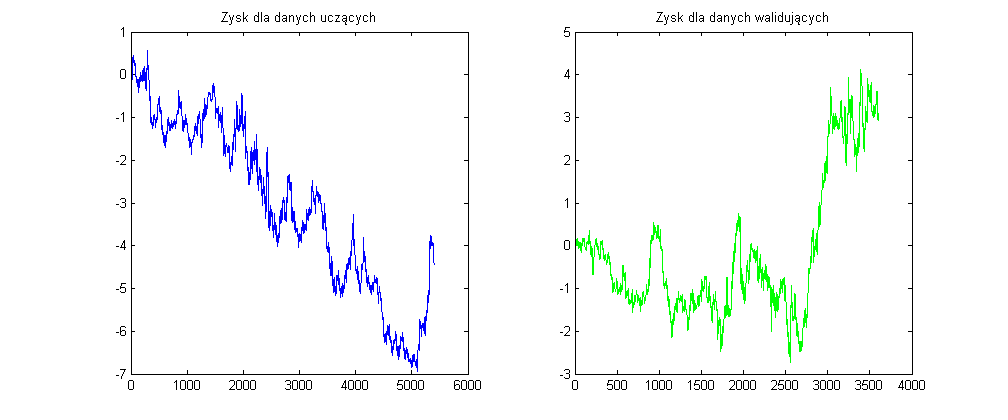
\includegraphics[scale=0.6]{SF_zysk_us.png}\\
\caption{Zysk}
\end{figure}
\FloatBarrier
\noindent \textbf{Wycinek ValK i ValD}\\
\begin{figure}[h!]
\centering
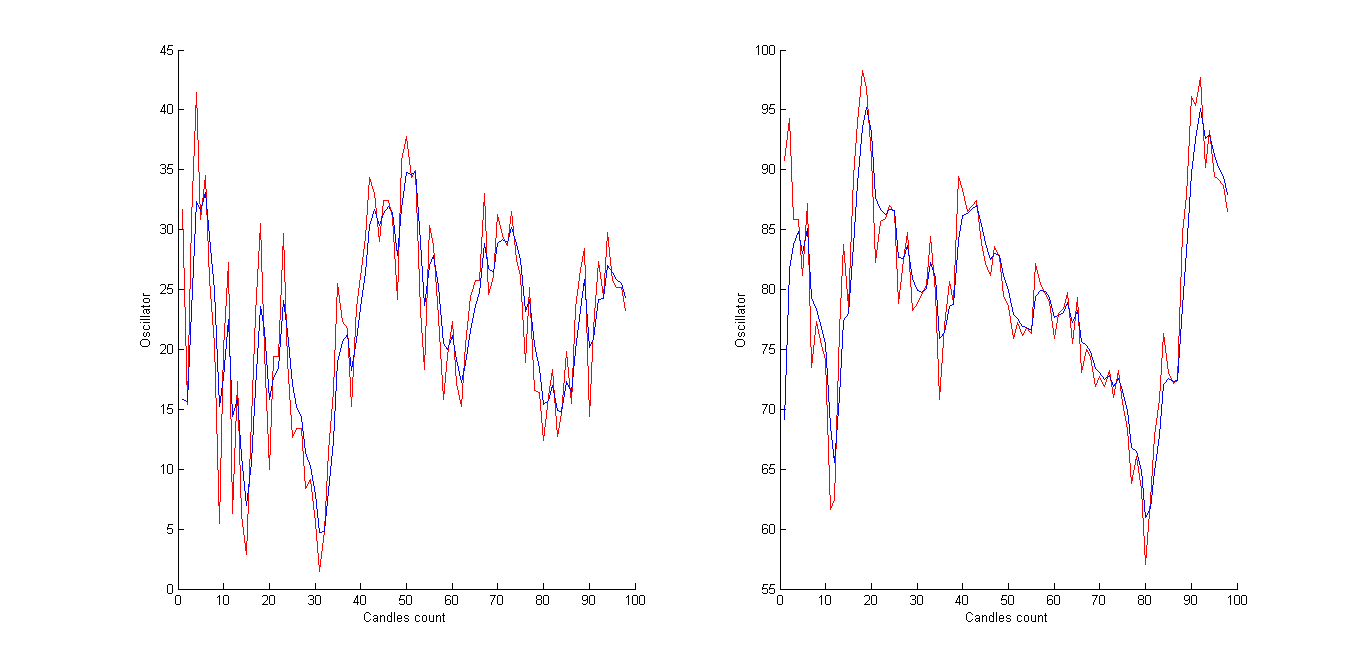
\includegraphics[scale=0.4]{ValD_ValK_us.png}
\caption{ValD - kolor niebieski, ValK - kolor czerowny }
\end{figure}
\FloatBarrier
%
